\subsection{Batcher's Bitonic Parallel Sorter}
Batcher's bitonic merger and sorter is a parallel sorting algorithm which has a good implementation in hardware. We have produced an implementation of this algorithm in Haskell originally for circuit generation for FPGAs. However, this executable model also represents an interesting software implicit parallelization exercise because the entire parallel structure of the algorithm is expressed in terms of just one combinator called \codef{par2}:

\begin{lstlisting}
par2 :: (a -> b) -> (c -> d) -> (a, c) -> (b, d)
par2 circuit1 circuit2 (input1, input2)
  = (output1, output2)
    where
    output1 = circuit1 input1
    output2 = circuit2 input2
\end{lstlisting}

This combinator captures the idea of two circuits which are independent and execute in parallel. This combinator is used to define other combinators which express different ways of performing parallel divide and conquer operations:

\begin{lstlisting}
two :: ([a] -> [b]) -> [a] -> [b]
two r = halve >-> par2 r r >-> unhalve

ilv :: ([a] -> [b]) -> [a] -> [b]
ilv r = unriffle >-> two r >-> riffle
\end{lstlisting}

These combinators are in turn used to define a butterfly parallel processing network which describes a merger:

\begin{lstlisting}
butterfly circuit [x,y] = circuit [x,y]
butterfly circuit input
  = (ilv (butterfly circuit) >-> evens circuit) input
\end{lstlisting}

A column of par-wise processing elements is used to combine the results of two sub-merges:

\begin{lstlisting}
evens :: ([a] -> [b]) -> [a] -> [b]
evens f = chop 2 >-> map f >-> concat
\end{lstlisting}

This parallel Batcher's bitonic merger plus the \codef{evens} function can be used to build a parallel Batcher's bitonic sorter:

\begin{lstlisting}
sortB cmp [x, y] = cmp [x, y]
sortB cmp input
  = (two (sortB cmp) >-> sndList reverse >-> butterfly cmp) input
\end{lstlisting}


A straight-forward way to perform a semi-explicit parallelization of the \codef{par2} combinator is use \codef{par} to spark off the evaluation of one of the sub-circuits.

\begin{lstlisting}
par2 :: (a -> b) -> (c -> d) -> (a, c) -> (b, d)
par2 circuit1 circuit2 (input1, input2)
  = output1 `par` (output2 `pseq` (output1, output2))
    where
    output1 = circuit1 input1
    output2 = circuit2 input2
\end{lstlisting}

This relatively simple change results in a definite performance gain due to parallelism. Here is the log output produced by running a test-bench program with just one Haskell execution context:

\begin{verbatim}
.\bsortpar.exe +RTS -N1 -l -qg0 -qb -sbsortpar-N1.log
  SPARKS: 106496 (0 converted, 106496 pruned)

  INIT  time    0.00s  (  0.00s elapsed)
  MUT   time    5.32s  (  5.37s elapsed)
  GC    time    0.72s  (  0.74s elapsed)
  EXIT  time    0.00s  (  0.00s elapsed)
  Total time    6.04s  (  6.12s elapsed)
\end{verbatim}

Although many sparks are created non are taken up because there is only one worker thread. The execution trace for this invocation is shown in Figure~\ref{f:bsortpar-n1}.

\begin{figure*}
\begin{center}
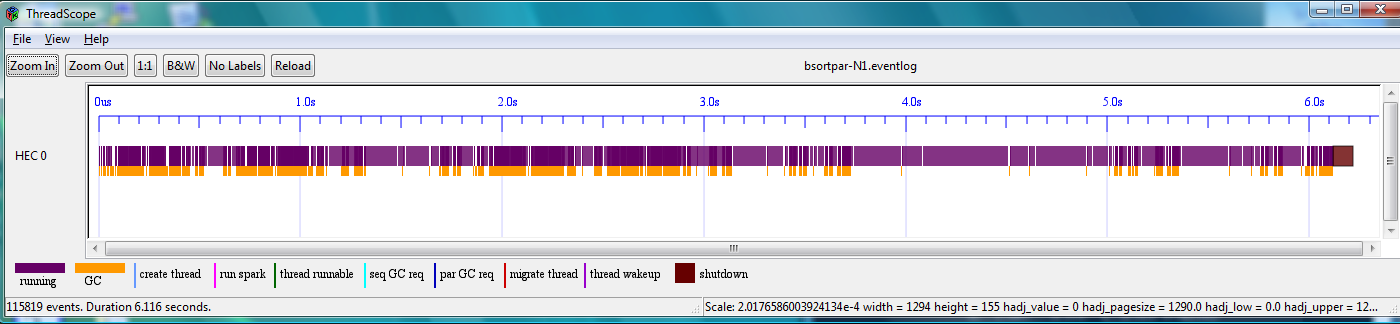
\includegraphics[width=17cm]{bsortpar-n1.png}
\end{center}
\caption{A sequential execution of bsort}
\label{f:bsortpar-n1}
\end{figure*}

\begin{figure*}
\begin{center}
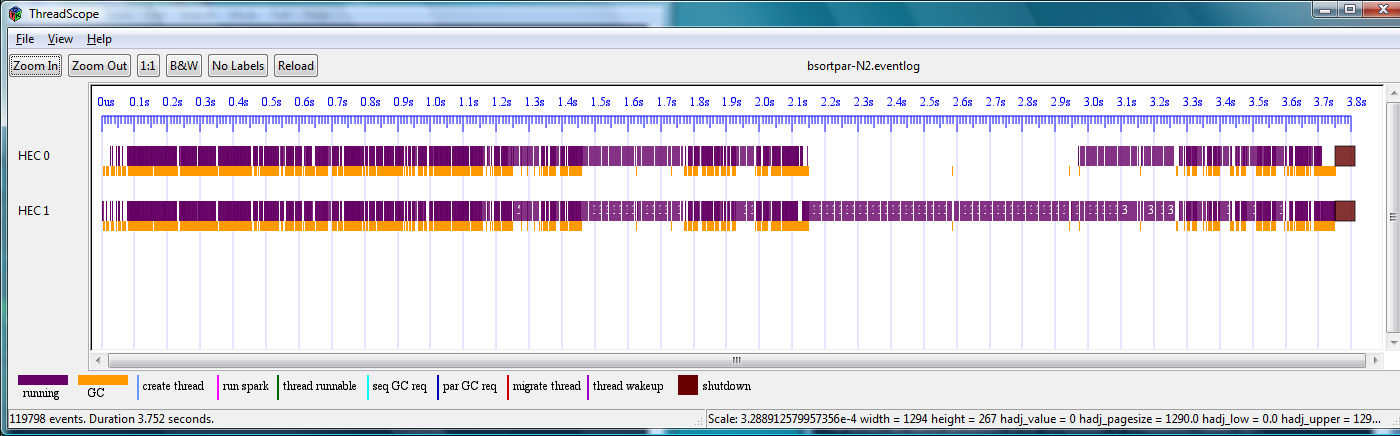
\includegraphics[width=17cm]{bsortpar-n2.png}
\end{center}
\caption{A parallel execution of bsort}
\label{f:bsortpar-n2}
\end{figure*}

 Running with two threads shows a very good performance improvement:

\begin{verbatim}
$ cat bsortpar-N2.log
.\bsortpar.exe +RTS -N2 -l -qg0 -qb -sbsortpar-N2.log
  SPARKS: 106859 (49 converted, 106537 pruned)

  INIT  time    0.00s  (  0.00s elapsed)
  MUT   time    4.73s  (  3.03s elapsed)
  GC    time    1.64s  (  0.72s elapsed)
  EXIT  time    0.00s  (  0.00s elapsed)
  Total time    6.36s  (  3.75s elapsed)
\end{verbatim}

This example produces very many sparks most of which fizzle but enough sparks are turned into productive work i.e. 6.36 seconds worth of work done in 3.75 seconds of time. The execution trace for this invocation is shown in Figure~\ref{f:bsortpar-n2}. 
There is an obvious sequential block of execution between 2.1 seconds and 2.9 seconds and this is due to a sequential component of the algorithm which combines the results of parallel sub-computations i.e the \codef{evens} function. We can use the parallel stratagies library to change the sequential application in the definition of \codef{evens} to a parallel map operation:

\begin{lstlisting}
evens :: ([a] -> [b]) -> [a] -> [b]
evens f = chop 2 >-> parMap rwhnf f >-> concat
\end{lstlisting}

This results in many more sparks being converted:

\begin{lstlisting}
.\bsortpar2.exe +RTS -N2 -l -qg0 -qb -sbsortpar2-N2.log
  SPARKS: 852737 (91128 converted, 10175 pruned)

  INIT  time    0.00s  (  0.04s elapsed)
  MUT   time    4.95s  (  3.86s elapsed)
  GC    time    1.29s  (  0.65s elapsed)
  EXIT  time    0.00s  (  0.00s elapsed)
  Total time    6.24s  (  4.55s elapsed)
\end{lstlisting}

